
\section{Numerical examples}\label{examples}
\DIFdelbegin \DIFdel{The suggested method , which uses }\DIFdelend \DIFaddbegin \DIFadd{In this section, the suggested method is validated through several examples using the }\DIFaddend Nitsche's method, the consistent reproducing kernel gradient smoothing integration scheme (RKGSI), and the non-consistent Gauss integration scheme (GI) with penalty method, as well as the proposed Hu-Washizu formulation (HW) to enforce the necessary boundary conditions\DIFdelbegin \DIFdel{, is validated in this section through several examples}\DIFdelend . A normalized support size of 2.5 is used for all the \DIFaddbegin \DIFadd{considered }\DIFaddend methods to ensure the requirement of quadratic base meshfree approximation. To eliminate the influence of integration \DIFaddbegin \DIFadd{error}\DIFaddend , the Gauss integration scheme uses 6 Gauss points for domain integration and 3 points for boundary integration, so as to maintain the same integration accuracy between domain and boundaries. Moreover, the number of integration points are identical between the Gauss and RKGSI schemes. The error estimates of displacement ($L_2$-Error) and energy ($H_e$-Error) is used here:
\begin{equation}
\begin{split}
L_2\text{-Error} &= \frac{\sqrt{\int_\Omega(\boldsymbol v - \boldsymbol v^h) \cdot (\boldsymbol v - \boldsymbol v^h)d\Omega}}{\sqrt{\boldsymbol v \cdot \boldsymbol v}} \\
H_e\text{-Error} &= \frac{\sqrt{\int_\Omega \left ((\varepsilon_{\alpha\beta} - \varepsilon_{\alpha\beta}^h)(N^{\alpha\beta} - N^{\alpha\beta h}) + \int_\Omega(\kappa_{\alpha\beta}-\kappa_{\alpha\beta}^h)(M^{\alpha\beta}-M^{\alpha\beta h}) \right )d\Omega}}{\sqrt{\int_\Omega(\varepsilon_{\alpha\beta}N^{\alpha\beta} + \kappa_{\alpha\beta}M^{\alpha\beta})d\Omega}}
\end{split}
\end{equation}

\subsection{Patch tests}
The linear and quadratic patch tests for flat and curved thin shells are firstly studied to verify the variational consistency of the proposed method. As shown in Fig. \ref{ptf1}, the flat and curved models are depicted by an identical parametric domain $\Omega = (0,1)\otimes(0,1)$, where the cylindrical coordinate system with radius $R=1$\DIFaddbegin \DIFadd{, thickness $h=0.1$ }\DIFaddend is employed to describe the curved model, and the whole domain $\Omega$ is discretized by the $165$ meshfree nodes. \DIFaddbegin \DIFadd{The Young's modulus and Poisson's ratio of thin shell are set to $E=1$, $\nu=0$. The artificial parameters of $\alpha_v=10^5\times E$, $\alpha_\theta=10^3\times E$, $\alpha_C=10^5\times E$ and $\alpha_v=10^9\times E, \alpha_\theta=10^9\times E, \alpha_C=10^9\times E$ were adopted in Nitsche's- and penalty- method, respectively. }\DIFaddend All the boundaries are enforced as essential boundary conditions with the following manufactured exact solution:
\begin{equation}
\boldsymbol v = \begin{Bmatrix}
(\xi^1+2\xi^2)^n \\ (3\xi^1+4\xi^2)^n \\ (5\xi^1+6\xi^2)^n
\end{Bmatrix},\quad
n = \begin{cases}
1 & \text{Linear patch test} \\
2 & \text{Quadratic patch test}
\end{cases}
\end{equation}

\begin{figure}[!ht]
    \centering
    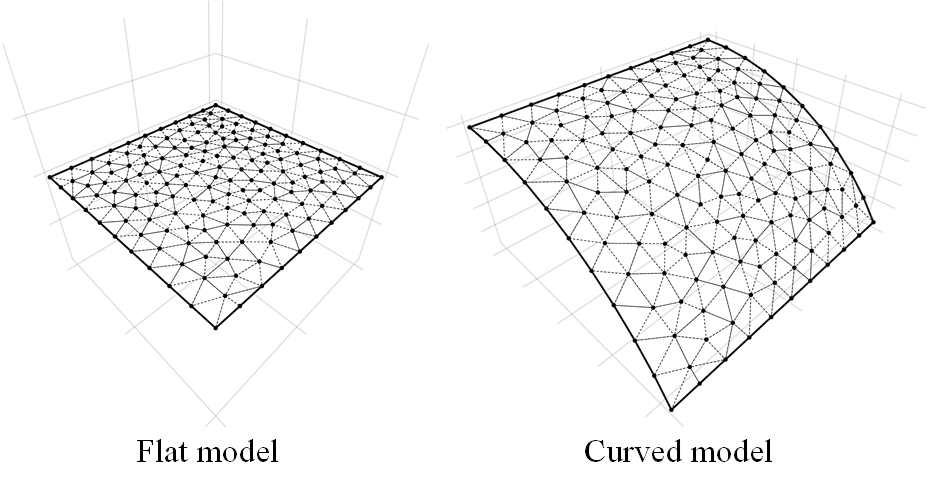
\includegraphics[width=\textwidth]{figures/ptmsh}
    \caption{Meshfree discretization for patch test}\label{ptf1}
\end{figure}

Table \ref{ptt1} lists the $L_2$- and $H_e$-Error results of patch test with flat model, where the RKGSI scheme with variational consistent essential boundary enforcement, i.e. RKGSI-Nitsche and RKGSI-HW, can pass the linear and quadratic patch test. \DIFaddbegin \DIFadd{In contrast, the RKGSI-Penalty cannot pass the patch test since the Penalty method is unable to ensure the variational consistency. }\DIFaddend Due to the loss of variational consistency condition, even with \DIFaddbegin \DIFadd{the }\DIFaddend Nitsche's method, Gauss meshfree formulations show noticeable errors. Table \ref{ptt2} shows the results for curved model, which indicated that all the considered methods cannot pass the patch test. This is mainly because the proposed smoothed gradient of Eqs. (\ref{approxse1}) and (\ref{approxse2}) could not exactly reproduce the non-polynomial membrane and bending \DIFdelbegin \DIFdel{stress. However}\DIFdelend \DIFaddbegin \DIFadd{stresses. On the other hand}\DIFaddend , the RKGSI-HW and RKGSI-Nitsche methods \DIFdelbegin \DIFdel{also }\DIFdelend provide better accuracy compared to \DIFdelbegin \DIFdel{others }\DIFdelend \DIFaddbegin \DIFadd{the other approaches }\DIFaddend due to the fulfillment of first second-order variational consistency. \DIFaddbegin \DIFadd{Even only with local variational consistency, the RKGSI-Penalty obtained a better result than the traditional Gauss scheme. }\DIFaddend Meanwhile, the bending moment contours of $M^{12}$ are listed in Fig. \ref{ptf2}, which further verify that the proposed method provided a satisfactory result compared to \DIFaddbegin \DIFadd{the }\DIFaddend exact solution. \DIFdelbegin \DIFdel{On the other hand, the }\DIFdelend \DIFaddbegin \DIFadd{Contrarily, both the RKGSI-Penalty and the }\DIFaddend conventional Gauss meshree formulations \DIFdelbegin \DIFdel{showed }\DIFdelend \DIFaddbegin \DIFadd{observed }\DIFaddend errors.

\begin{table}[!ht]
\centering
\caption{Results of patch test for flat model.}\label{ptt1}
\begin{tabular}{lcccc}
\toprule
 & \multicolumn{2}{c}{Linear patch test} & \multicolumn{2}{c}{Quadratic patch test} \\ \cline{2-5}
 & $L_2$-Error & $H_e$-Error & $L_2$-Error & $H_e$-Error \\
    \midrule
    GI-Penalty & \DIFdelbeginFL \DIFdelFL{$4.45E-4$ }\DIFdelendFL \DIFaddbeginFL \DIFaddFL{4.45E-04 }\DIFaddendFL & \DIFdelbeginFL \DIFdelFL{$1.35E-2$ }\DIFdelendFL \DIFaddbeginFL \DIFaddFL{1.35E-02 }\DIFaddendFL & \DIFdelbeginFL \DIFdelFL{$2.01E-3$ }\DIFdelendFL \DIFaddbeginFL \DIFaddFL{2.01E-03 }\DIFaddendFL & \DIFdelbeginFL \DIFdelFL{$1.63E-2$ }\DIFdelendFL \DIFaddbeginFL \DIFaddFL{1.63E-02 }\DIFaddendFL \\
    GI-Nitsche & \DIFdelbeginFL \DIFdelFL{$4.51E-4$ }\DIFdelendFL \DIFaddbeginFL \DIFaddFL{4.51E-04 }\DIFaddendFL & \DIFdelbeginFL \DIFdelFL{$1.42E-2$ }\DIFdelendFL \DIFaddbeginFL \DIFaddFL{1.42E-02 }\DIFaddendFL & \DIFdelbeginFL \DIFdelFL{$1.22E-3$ }\DIFdelendFL \DIFaddbeginFL \DIFaddFL{1.22E-03 }\DIFaddendFL & \DIFdelbeginFL \DIFdelFL{$1.68E-2$ }\DIFdelendFL \DIFaddbeginFL \DIFaddFL{1.68E-02 }\DIFaddendFL \\
    RKGSI-Penalty & \DIFdelbeginFL \DIFdelFL{$3.64E-9$ }\DIFdelendFL \DIFaddbeginFL \DIFaddFL{3.64E-09 }\DIFaddendFL & \DIFdelbeginFL \DIFdelFL{$6.77E-8$ }\DIFdelendFL \DIFaddbeginFL \DIFaddFL{6.77E-08 }\DIFaddendFL & \DIFdelbeginFL \DIFdelFL{$4.54E-9$ }\DIFdelendFL \DIFaddbeginFL \DIFaddFL{4.54E-09 }\DIFaddendFL & \DIFdelbeginFL \DIFdelFL{$6.57E-8$ }\DIFdelendFL \DIFaddbeginFL \DIFaddFL{6.57E-08 }\DIFaddendFL \\
    RKGSI-Nitsche & \DIFdelbeginFL \DIFdelFL{$3.31E-12$ }\DIFdelendFL \DIFaddbeginFL \DIFaddFL{3.31E-12 }\DIFaddendFL & \DIFdelbeginFL \DIFdelFL{$1.34E-11$ }\DIFdelendFL \DIFaddbeginFL \DIFaddFL{1.34E-11 }\DIFaddendFL & \DIFdelbeginFL \DIFdelFL{$5.98E-12$ }\DIFdelendFL \DIFaddbeginFL \DIFaddFL{5.98E-12 }\DIFaddendFL & \DIFdelbeginFL \DIFdelFL{$1.21E-11$ }\DIFdelendFL \DIFaddbeginFL \DIFaddFL{1.21E-11 }\DIFaddendFL \\
    RKGSI-HR & \DIFdelbeginFL \DIFdelFL{$6.67E-13$ }\DIFdelendFL \DIFaddbeginFL \DIFaddFL{6.67E-13 }\DIFaddendFL & \DIFdelbeginFL \DIFdelFL{$1.50E-11$ }\DIFdelendFL \DIFaddbeginFL \DIFaddFL{1.50E-11 }\DIFaddendFL & \DIFdelbeginFL \DIFdelFL{$1.07E-12$ }\DIFdelendFL \DIFaddbeginFL \DIFaddFL{1.07E-12 }\DIFaddendFL & \DIFdelbeginFL \DIFdelFL{$1.26E-11$ }\DIFdelendFL \DIFaddbeginFL \DIFaddFL{1.26E-11 }\DIFaddendFL \\
    \bottomrule
\end{tabular}
\end{table}

\begin{table}[!ht]
\centering
\caption{Results of patch test for cylindrical model.}\label{ptt2}
\begin{tabular}{lcccc}
\toprule
 & \multicolumn{2}{c}{Linear patch test} & \multicolumn{2}{c}{Quadratic patch test} \\ \cline{2-5}
 & $L_2$-Error & $H_e$-Error & $L_2$-Error & $H_e$-Error \\
    \midrule
    GI-Penalty & \DIFdelbeginFL \DIFdelFL{$3.79E-4$ }\DIFdelendFL \DIFaddbeginFL \DIFaddFL{3.79E-04 }\DIFaddendFL & \DIFdelbeginFL \DIFdelFL{$1.30E-2$ }\DIFdelendFL \DIFaddbeginFL \DIFaddFL{1.30E-02 }\DIFaddendFL & \DIFdelbeginFL \DIFdelFL{$1.74E-3$ }\DIFdelendFL \DIFaddbeginFL \DIFaddFL{1.74E-03 }\DIFaddendFL & \DIFdelbeginFL \DIFdelFL{$1.37E-2$ }\DIFdelendFL \DIFaddbeginFL \DIFaddFL{1.37E-02 }\DIFaddendFL \\
    GI-Nitsche & \DIFdelbeginFL \DIFdelFL{$4.04E-4$ }\DIFdelendFL \DIFaddbeginFL \DIFaddFL{4.04E-04 }\DIFaddendFL & \DIFdelbeginFL \DIFdelFL{$1.42E-2$ }\DIFdelendFL \DIFaddbeginFL \DIFaddFL{1.42E-02 }\DIFaddendFL & \DIFdelbeginFL \DIFdelFL{$1.15E-3$ }\DIFdelendFL \DIFaddbeginFL \DIFaddFL{1.15E-03 }\DIFaddendFL & \DIFdelbeginFL \DIFdelFL{$1.49E-2$ }\DIFdelendFL \DIFaddbeginFL \DIFaddFL{1.49E-02 }\DIFaddendFL \\
    RKGSI-Penalty & \DIFdelbeginFL \DIFdelFL{$1.47E-4$ }\DIFdelendFL \DIFaddbeginFL \DIFaddFL{1.47E-04 }\DIFaddendFL & \DIFdelbeginFL \DIFdelFL{$5.39E-3$ }\DIFdelendFL \DIFaddbeginFL \DIFaddFL{5.39E-03 }\DIFaddendFL & \DIFdelbeginFL \DIFdelFL{$2.26E-4$ }\DIFdelendFL \DIFaddbeginFL \DIFaddFL{2.26E-04 }\DIFaddendFL & \DIFdelbeginFL \DIFdelFL{$2.09E-3$ }\DIFdelendFL \DIFaddbeginFL \DIFaddFL{2.09E-03 }\DIFaddendFL \\
    RKGSI-Nitsche & \DIFdelbeginFL \DIFdelFL{$2.41E-6$ }\DIFdelendFL \DIFaddbeginFL \DIFaddFL{2.41E-06 }\DIFaddendFL & \DIFdelbeginFL \DIFdelFL{$7.37E-5$ }\DIFdelendFL \DIFaddbeginFL \DIFaddFL{7.37E-05 }\DIFaddendFL & \DIFdelbeginFL \DIFdelFL{$2.47E-6$ }\DIFdelendFL \DIFaddbeginFL \DIFaddFL{2.47E-06 }\DIFaddendFL & \DIFdelbeginFL \DIFdelFL{$2.89E-5$ }\DIFdelendFL \DIFaddbeginFL \DIFaddFL{2.89E-05 }\DIFaddendFL \\
    RKGSI-HR & \DIFdelbeginFL \DIFdelFL{$4.28E-6$ }\DIFdelendFL \DIFaddbeginFL \DIFaddFL{4.28E-06 }\DIFaddendFL & \DIFdelbeginFL \DIFdelFL{$1.30E-4$ }\DIFdelendFL \DIFaddbeginFL \DIFaddFL{1.30E-04 }\DIFaddendFL & \DIFdelbeginFL \DIFdelFL{$9.69E-6$ }\DIFdelendFL \DIFaddbeginFL \DIFaddFL{9.69E-06 }\DIFaddendFL & \DIFdelbeginFL \DIFdelFL{$2.41E-4$ }\DIFdelendFL \DIFaddbeginFL \DIFaddFL{2.41E-04 }\DIFaddendFL \\
    \bottomrule
\end{tabular}
\end{table}

\begin{figure}[!ht]
\centering
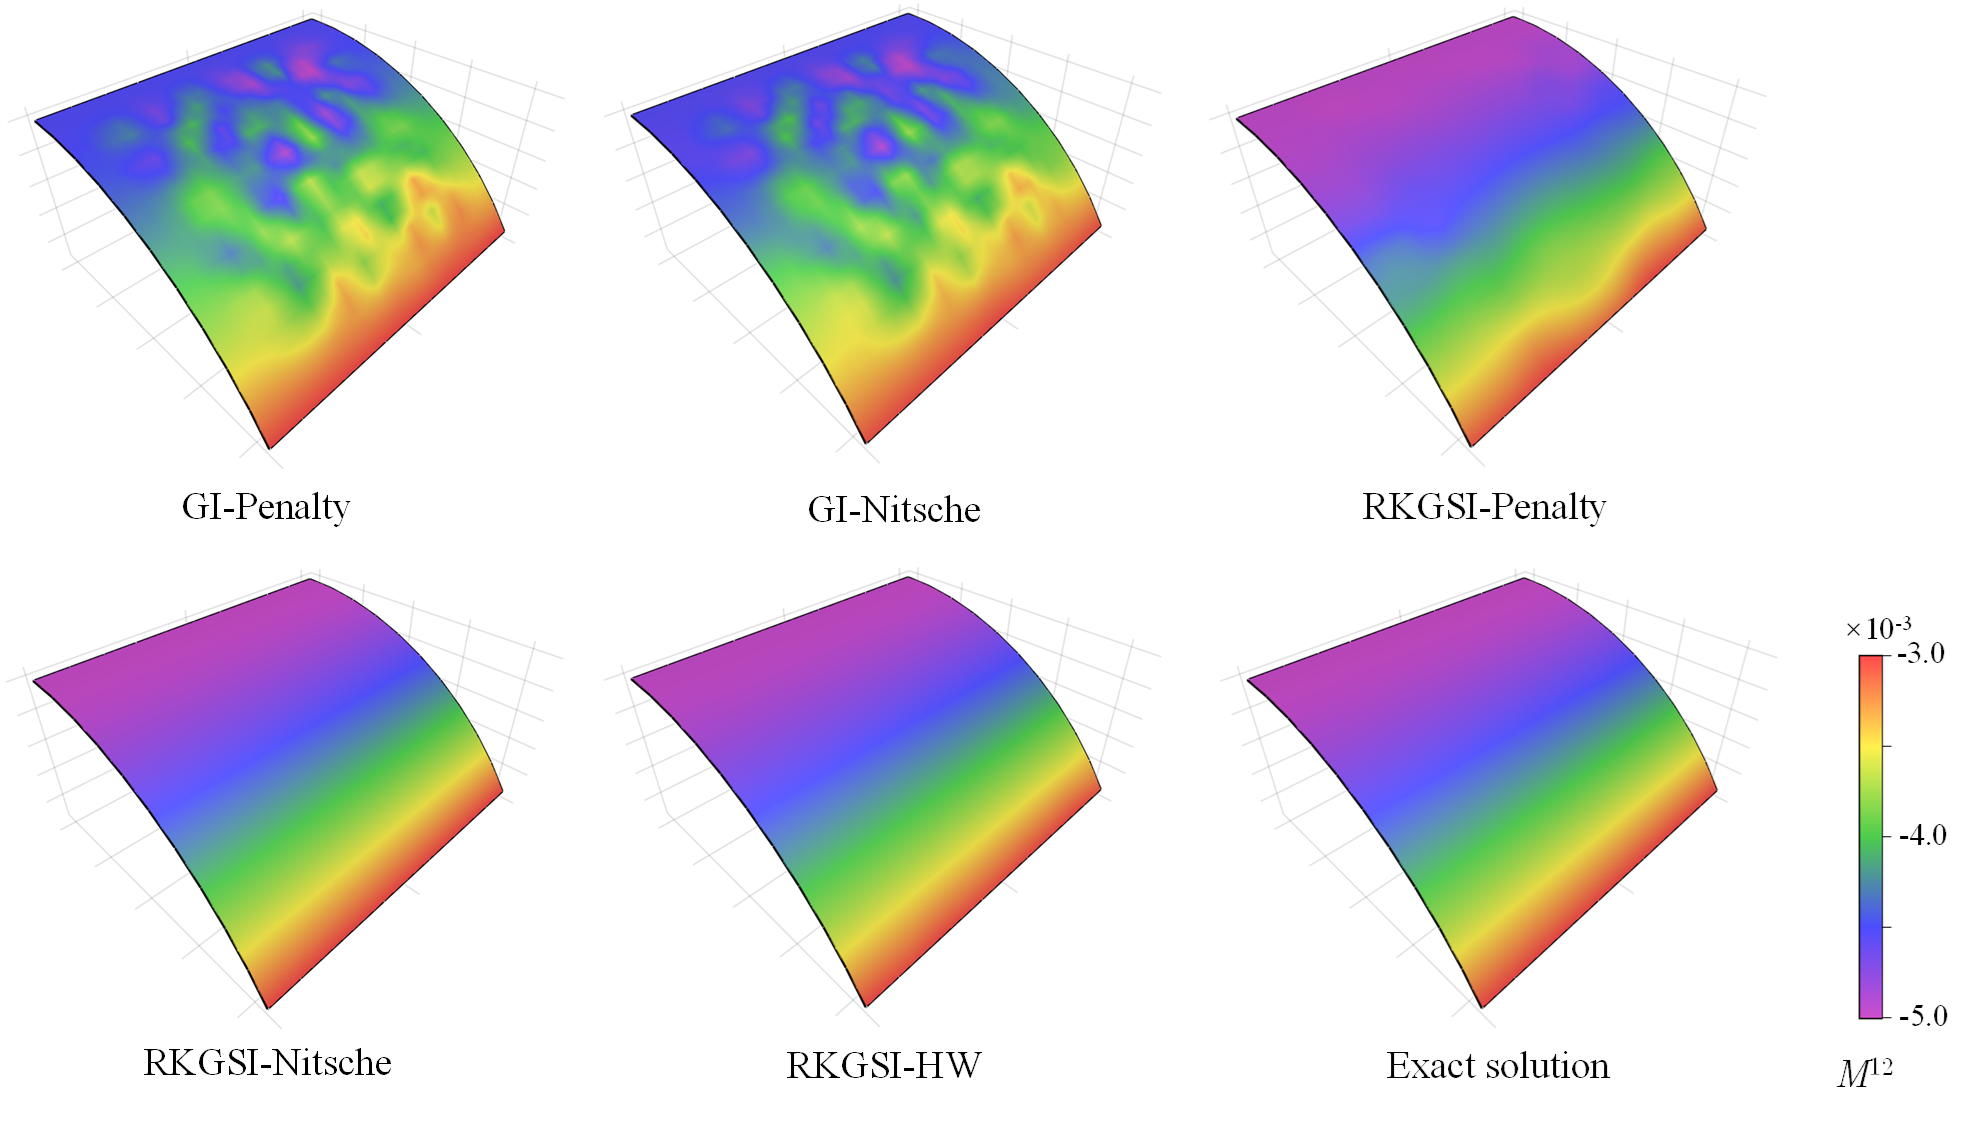
\includegraphics[width=\textwidth]{figures/ptc}
\caption{Contour plots of $M^{12}$ for curved shell patch test.}\label{ptf2}
\end{figure}

\subsection{Scordelis-Lo roof}
This example considers the classical Scordelis-Lo roof problem, as depicted in Fig. \ref{slf1}. The cylindrical roof has dimensions $R=25$, $L=50$, $h=0.25$, Young's modulus $E=4.32\times 10^8$ and Poisson's ratio $\nu=0.0$. The entire roof is subjected to an uniform body force of $b_z = -90$, with the straight edges remainning free and the the curved edges are enforced by $v_x=v_z=0$.

Due to the symmetry, only a quadrant of the model is considered for meshfree analysis, which is discretized by the $11\times 16$, $13\times 20$, $17\times 24$ and $19\times28$ meshfree nodes, as listed in Fig. \ref{slf2}. The comparison of the displacement in $z-$direction at node $A$, $v_{A3}$, is used as the investigated quantity, with the reference value \DIFdelbegin \DIFdel{0.3024 given by \mbox{%DIFAUXCMD
\cite{macneal1985}}\hskip0pt%DIFAUXCMD
}\DIFdelend \DIFaddbegin \DIFadd{0.3006 given by \mbox{%DIFAUXCMD
\cite{kiendl2009}}\hskip0pt%DIFAUXCMD
}\DIFaddend . Firstly, Fig. \ref{slf3} presents a sensitivity study for the artificial parameters of \DIFdelbegin \DIFdel{$\alpha_v$'s , }\DIFdelend \DIFaddbegin \DIFadd{$\alpha_{vi}$'s and }\DIFaddend $\alpha_\theta$'s in the RKGSI meshfree formulations with \DIFdelbegin \DIFdel{Nitsche's method and penalty method. }\DIFdelend \DIFaddbegin \DIFadd{the Nitsche's- and penalty- method, where all of the parameters are scaled by the support size as, $\alpha_{v\alpha} = s^{-1}\bar \alpha_v$, $\alpha_{v3} = s^{-3} \bar \alpha_v$ and $\alpha_\theta = s^{-1}\bar \alpha_\theta$. For a better comparison, the result of the proposed RKGSI-HW is also listed in this figure. }\DIFaddend The results of Fig. \ref{slf3} revealed, \DIFaddbegin \DIFadd{that }\DIFaddend Nitsche's method observed less artificial sensitivity. However, both the methods cannot trivially determine the optimal values of the artificial parameters. The optimal artificial parameters from Fig. \ref{slf3} are adopted for the convergence study in Fig. \ref{slf4}. The convergence result showed that the RKGSI \DIFaddbegin \DIFadd{method }\DIFaddend get satisfactory results while the traditional Gauss methods demonstrated noticeable errors.

\begin{figure}[!ht]
\centering
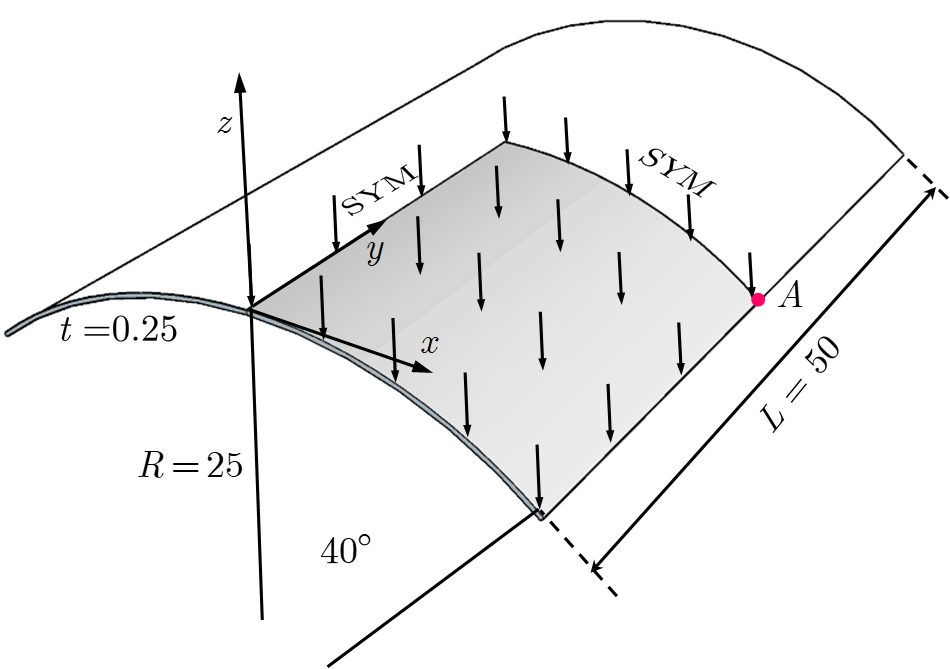
\includegraphics[width=0.7\textwidth]{figures/slm}
\caption{Description of Scordelis-Lo roof problem.}\label{slf1}
\end{figure}
\begin{figure}[!ht]
\centering
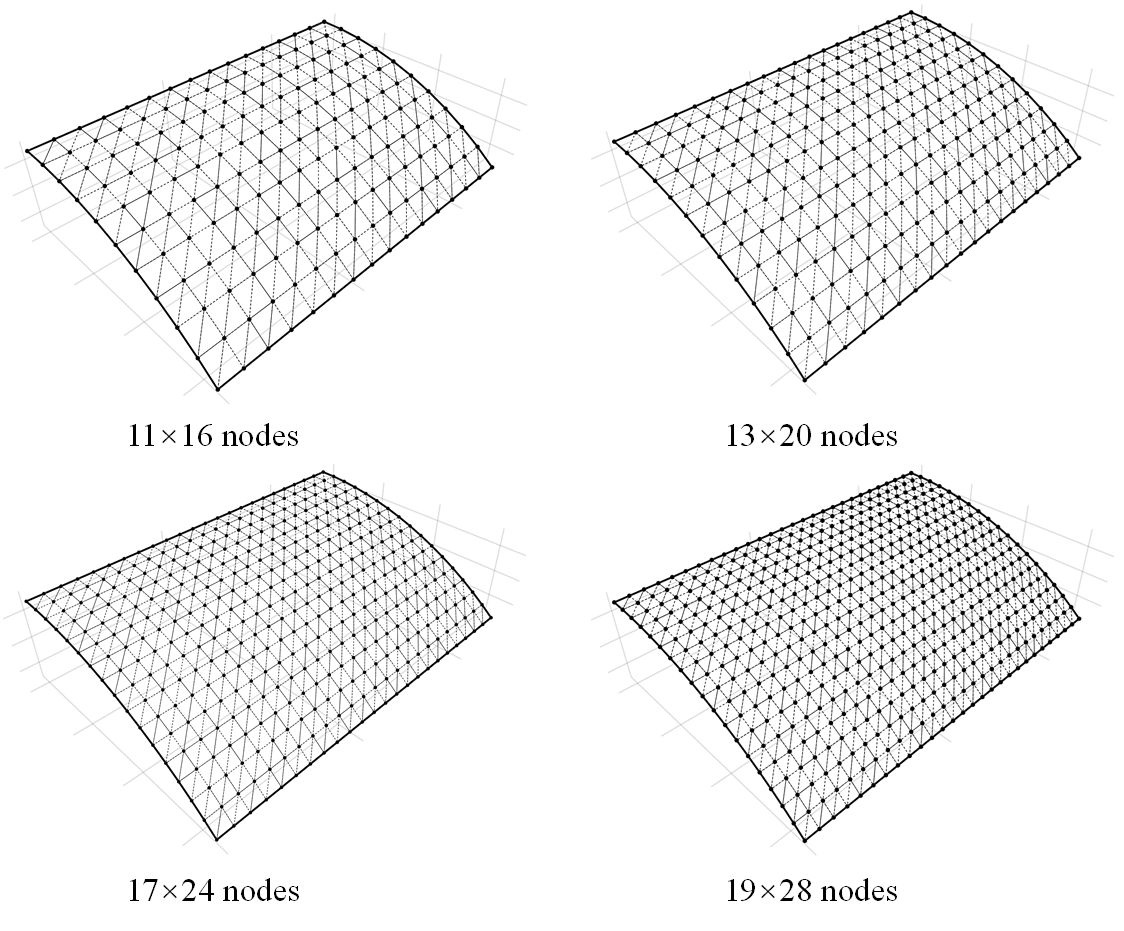
\includegraphics[width=\textwidth]{figures/slmsh}
\caption{Meshfree discretizations for Scordelis-Lo roof problem.}\label{slf2}
\end{figure}
\begin{figure}[!ht]
\centering
\DIFdelbeginFL %DIFDELCMD < 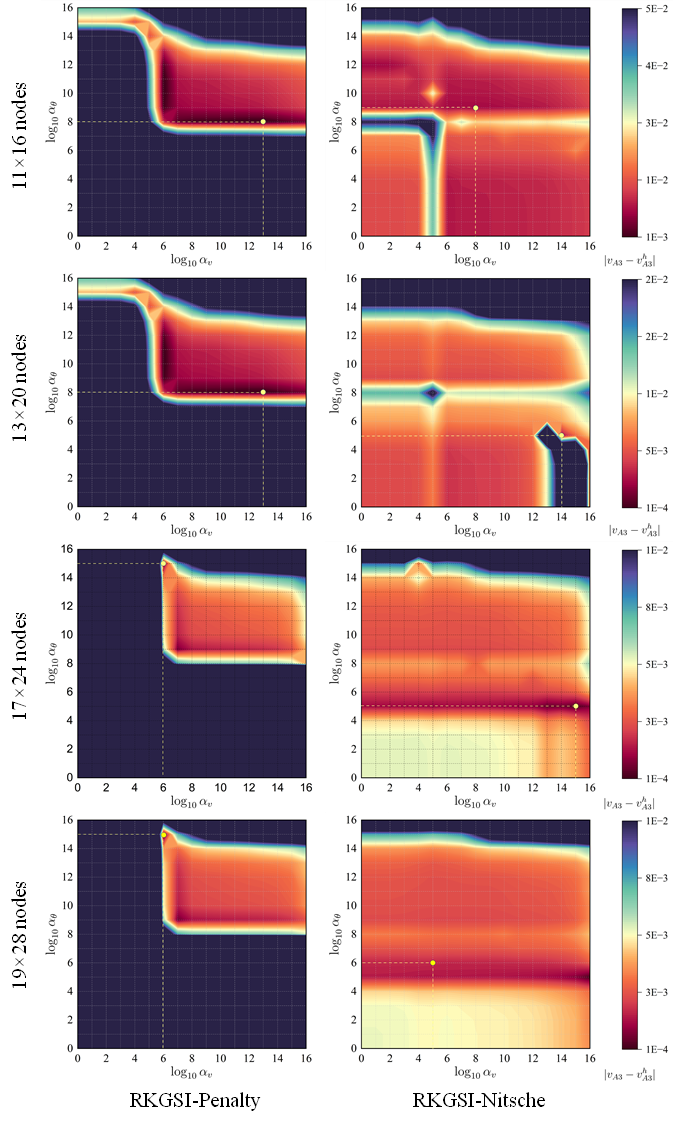
\includegraphics[width=\textwidth]{figures/sla}
%DIFDELCMD < %%%
\DIFdelendFL \DIFaddbeginFL 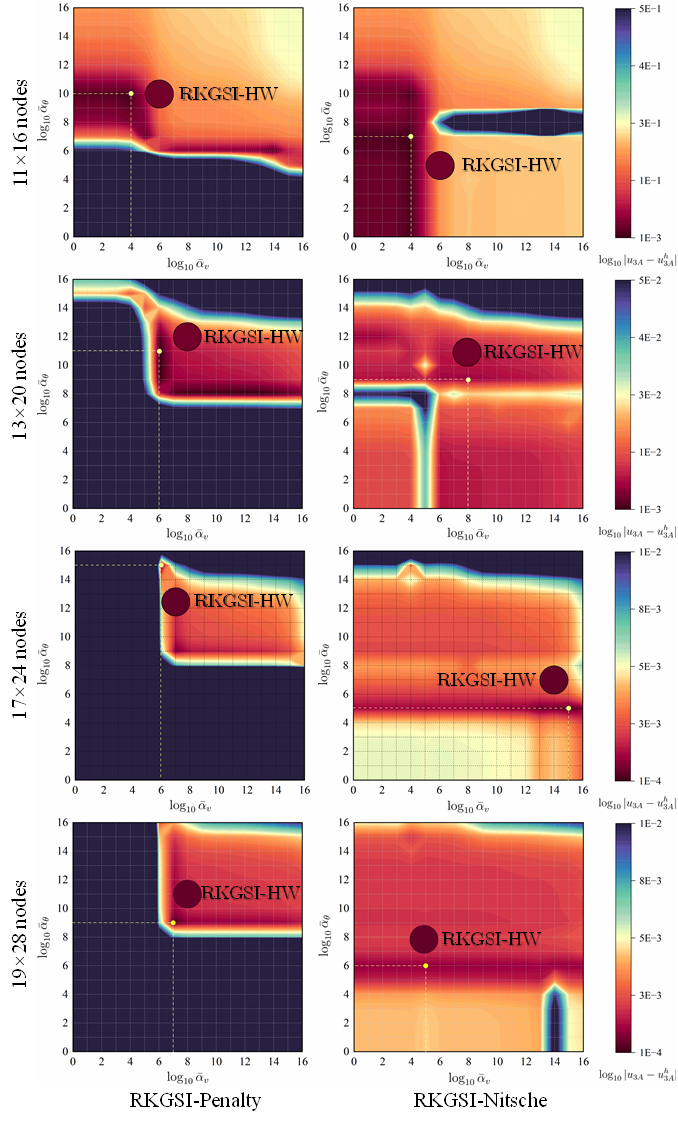
\includegraphics[width=\textwidth]{figures/sla_r1}
\DIFaddendFL \caption{Sensitivity comparison of $\alpha_v$ and $\alpha_\theta$ for Scordelis-Lo problem.}\label{slf3}
\end{figure}
\begin{figure}[!ht]
\centering
\DIFdelbeginFL %DIFDELCMD < 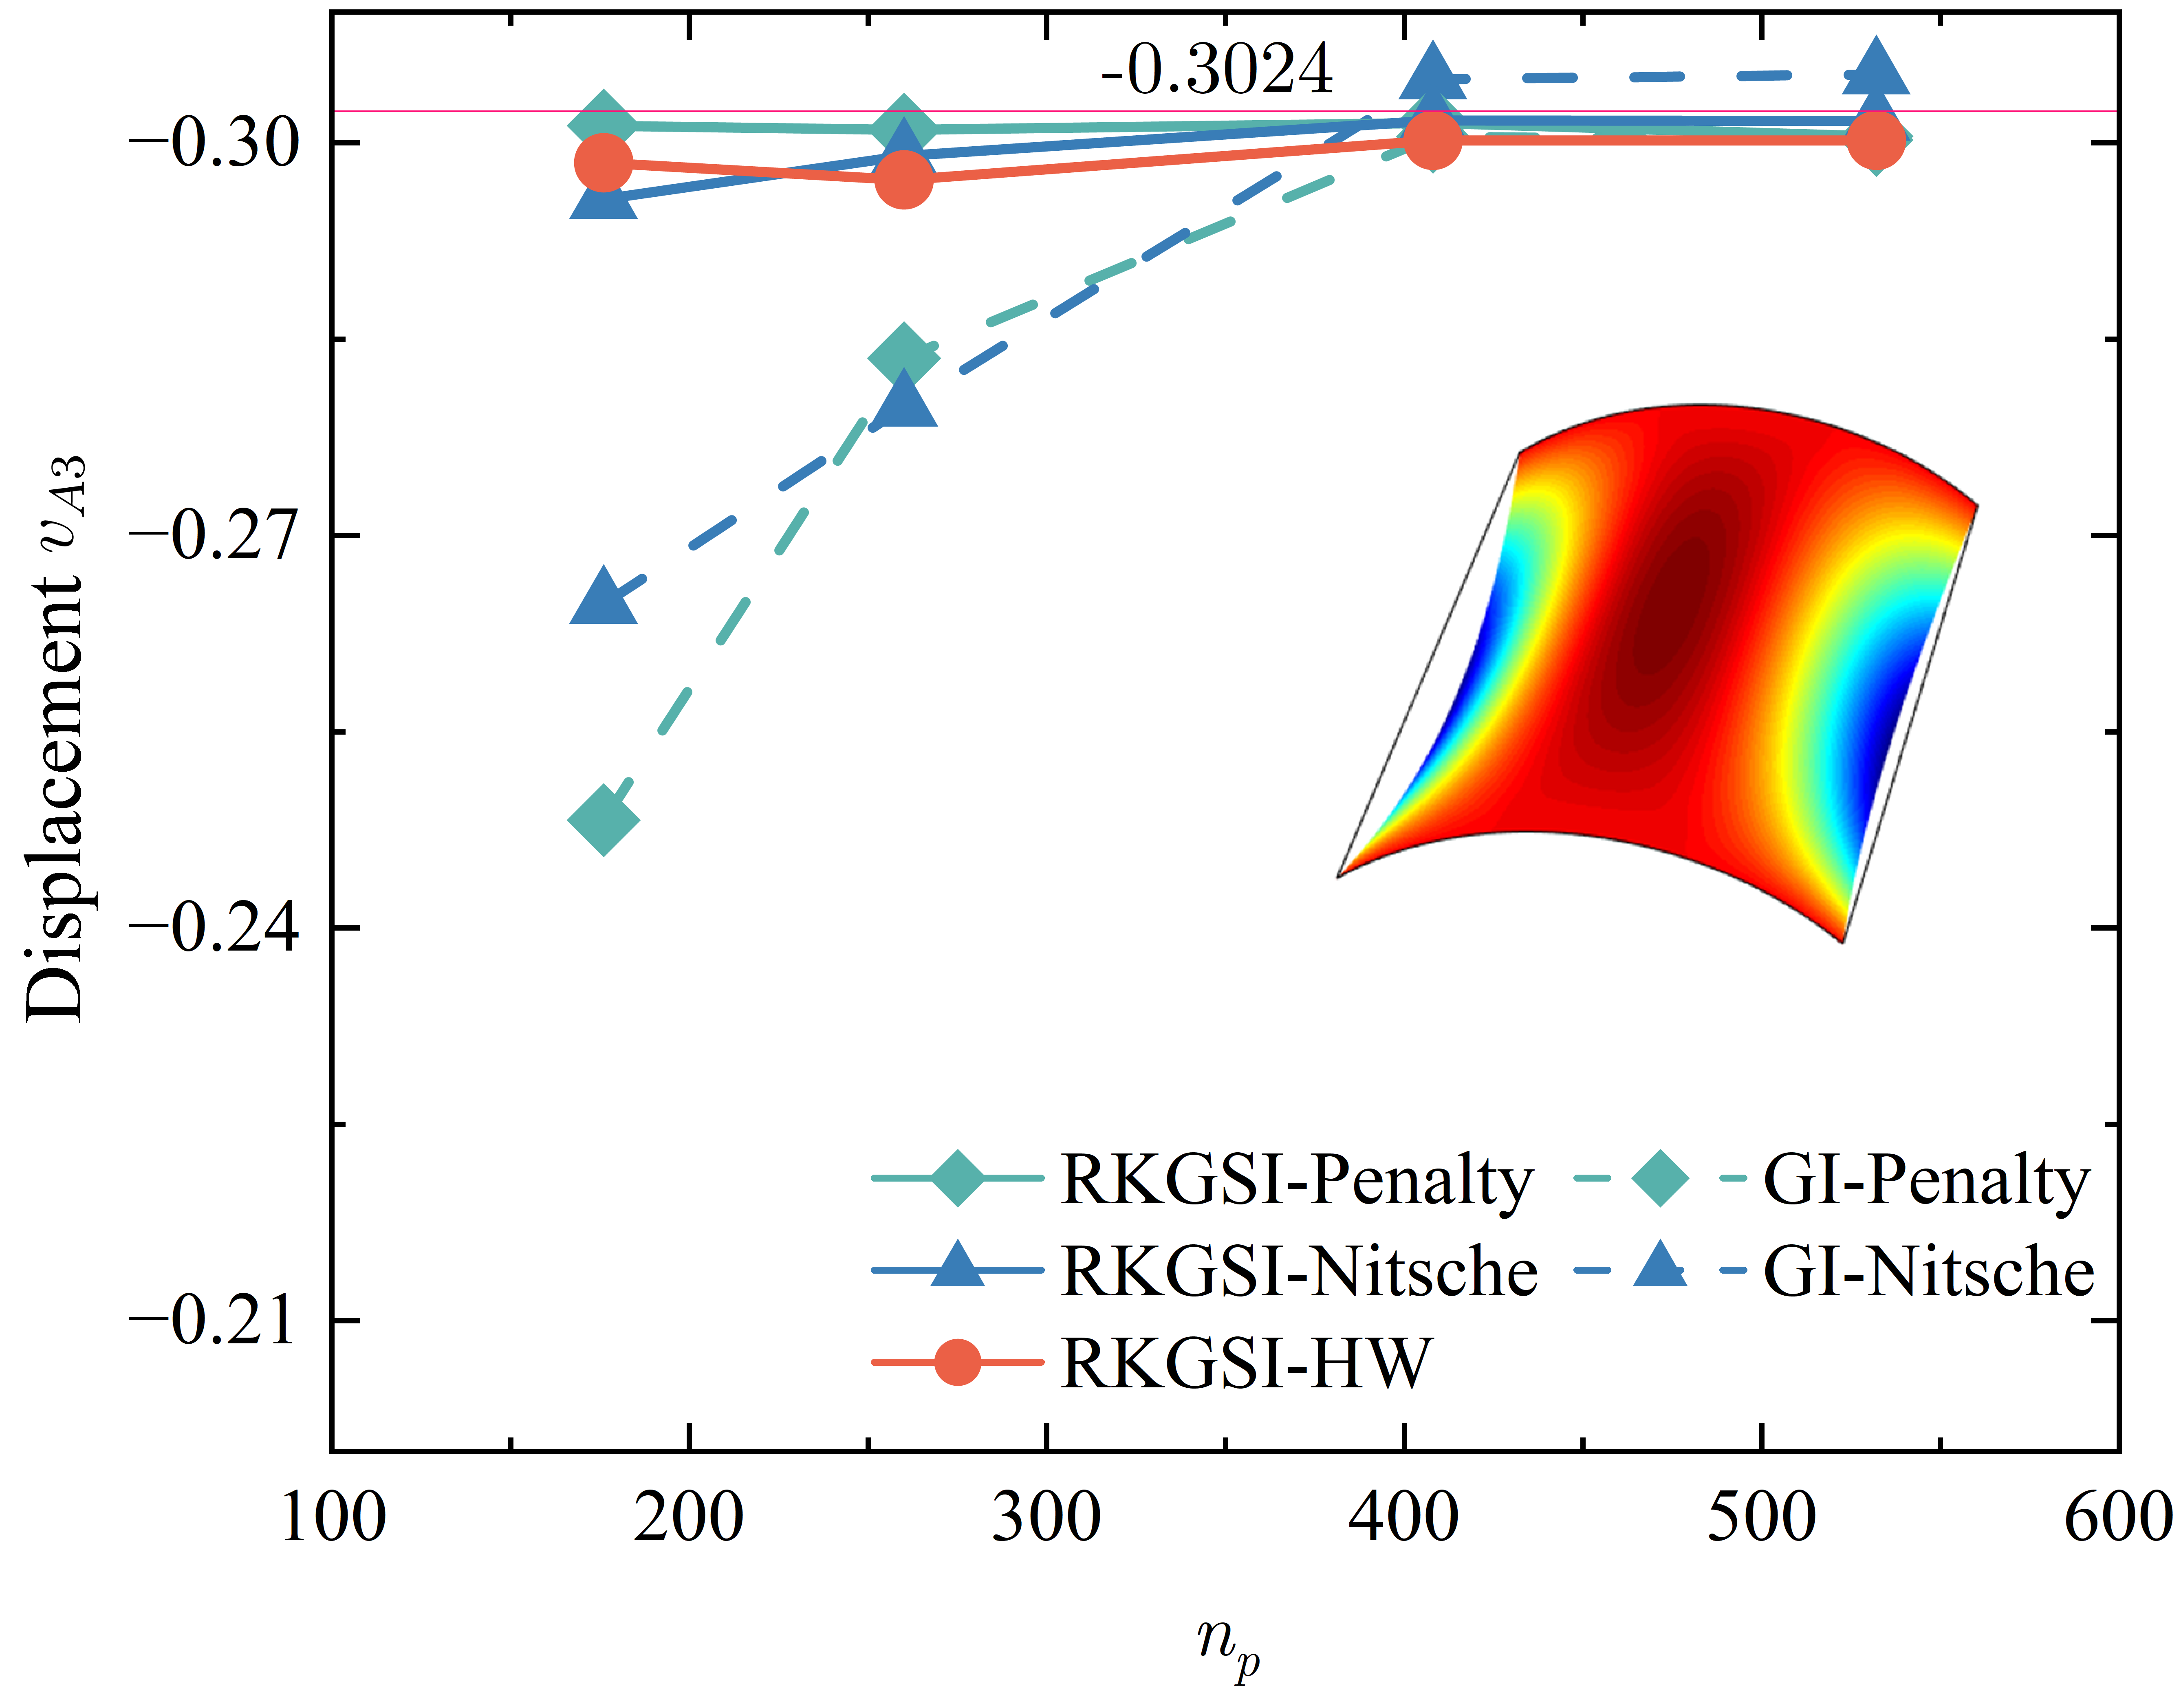
\includegraphics[width=\textwidth]{figures/sld}
%DIFDELCMD < %%%
\DIFdelendFL \DIFaddbeginFL 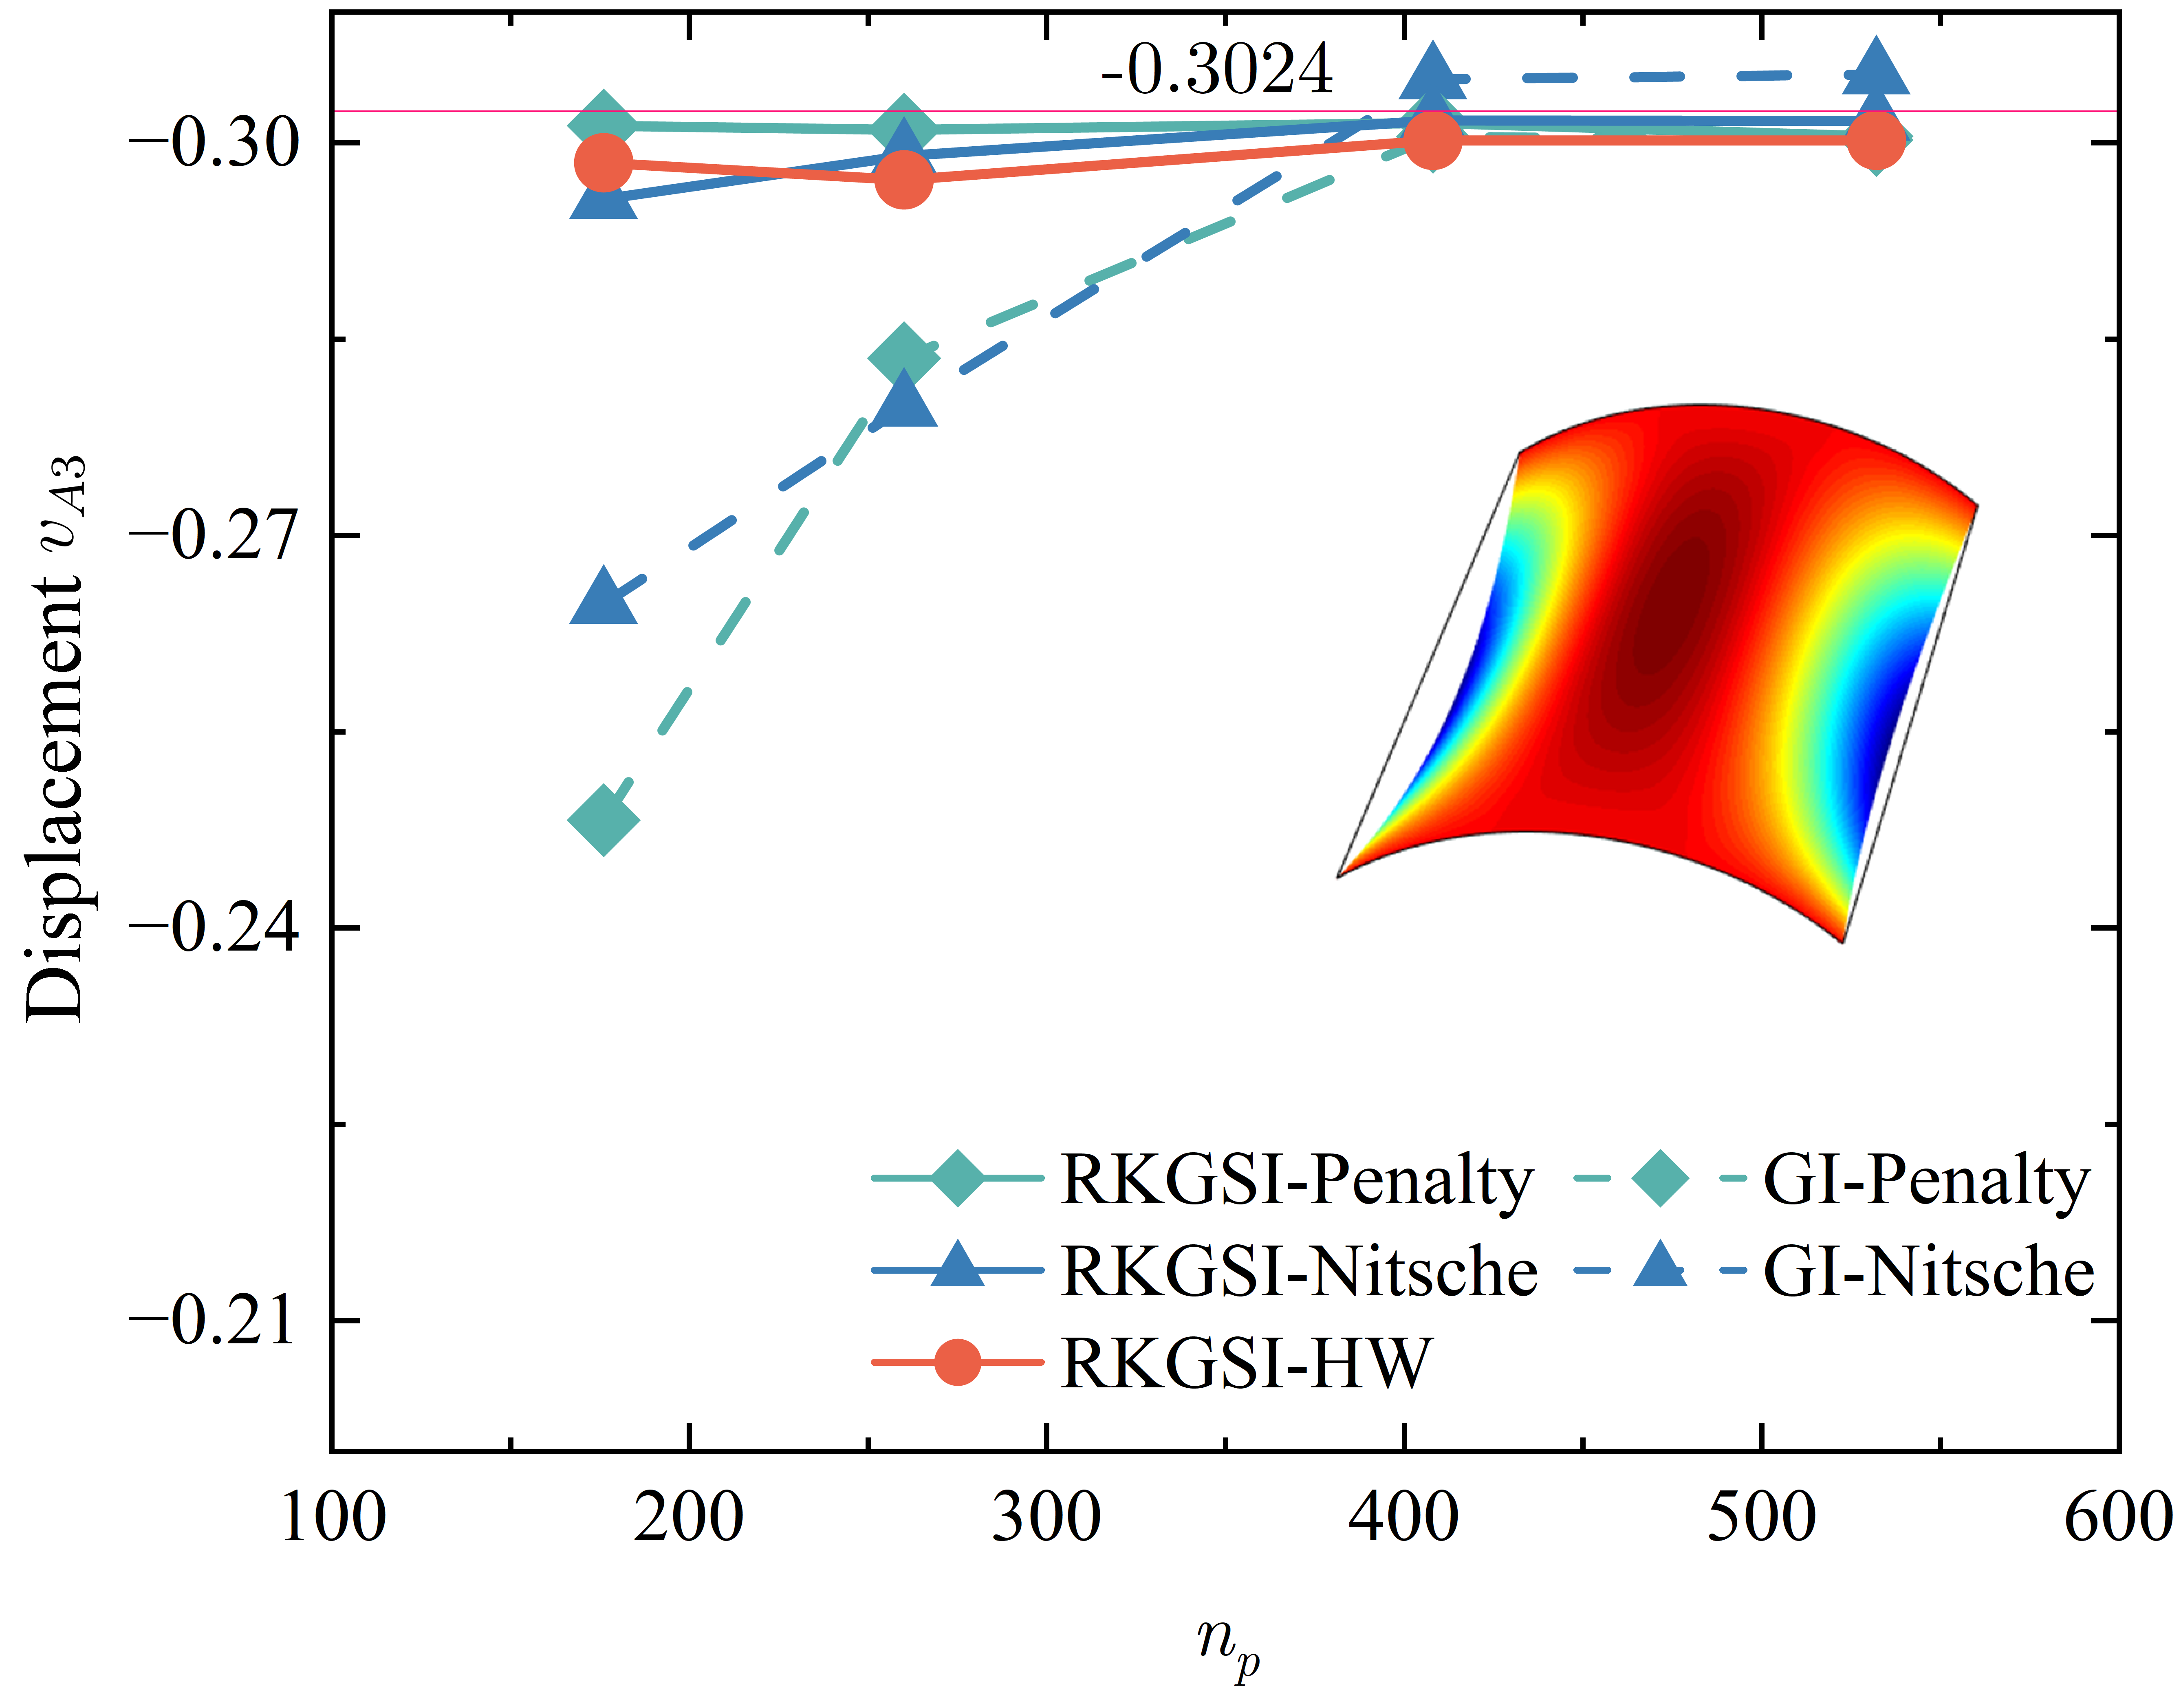
\includegraphics[width=\textwidth]{figures/sld_r1}
\DIFaddendFL \caption{Displacement convergence for Scordelis-Lo roof problem.}\label{slf4}
\end{figure}

\subsection{Pinched Hemispherical shell}
Consider the hemispherical shell shown in Fig. \ref{phf1}, which is loaded at four points $P=\pm 2$ at $90^\circ$ interval at its bottom. The hemispherical shell has an radius $R=10$, thickness $h=0.04$, Young's modulus $E=6.825\times10^7$ and Poisson's ratio $\nu = 0.3$.

Due to symmetry, only quadrant model, where the \DIFdelbegin \DIFdel{$8\times8$, }\DIFdelend $16\times16$, $24\times24$\DIFdelbegin \DIFdel{and }\DIFdelend \DIFaddbegin \DIFadd{, }\DIFaddend $32\times32$ \DIFaddbegin \DIFadd{and $40\times40$ }\DIFaddend meshfree nodes have been discretized \DIFdelbegin \DIFdel{, was }\DIFdelend \DIFaddbegin \DIFadd{as shown in Fig. (\ref{phfm}), were }\DIFaddend considered. The quantity under investigation for convergence is the displacement at \DIFdelbegin \DIFdel{$x-$direction }\DIFdelend \DIFaddbegin \DIFadd{$x$-direction }\DIFaddend on point $A$, $v_{A1}$ \DIFaddbegin \DIFadd{= 0.094 \mbox{%DIFAUXCMD
\cite{macneal1985}}\hskip0pt%DIFAUXCMD
}\DIFaddend .
Fig. \ref{phf2} displays the corresponding convergence results, indicating the RKGSI scheme performed significantly better compared to the GI meshfree formulation. Meanwhile, the efficiency comparison for this problem is also shown in Fig. \ref{phf3}, in which the CPU time for assembly and calculation of shape functions are considered. Fig. \ref{phf3}(a) indicates that the RKGSI scheme observed high efficiency in assembly. This is due to the variational inconsistent Gauss meshfree formulation which require more Gaussian points to get satisfactory results. Fig. \ref{phf3}(b) lists the CPU time spent on enforcing essential boundary conditions for the penalty method, Nitsche's method and proposed HW method. The results highlighted that the proposed HW method consumed comparable CPU time in assembly compared to Nitsche's method. However, less time was spent to calculate the shape functions. Since both the HW method and penalty method were developed considering the shape functions first order derivatives. For this reason, both the methods shared an almost identical time in computing the shape functions.
\begin{figure}[!ht]
\centering
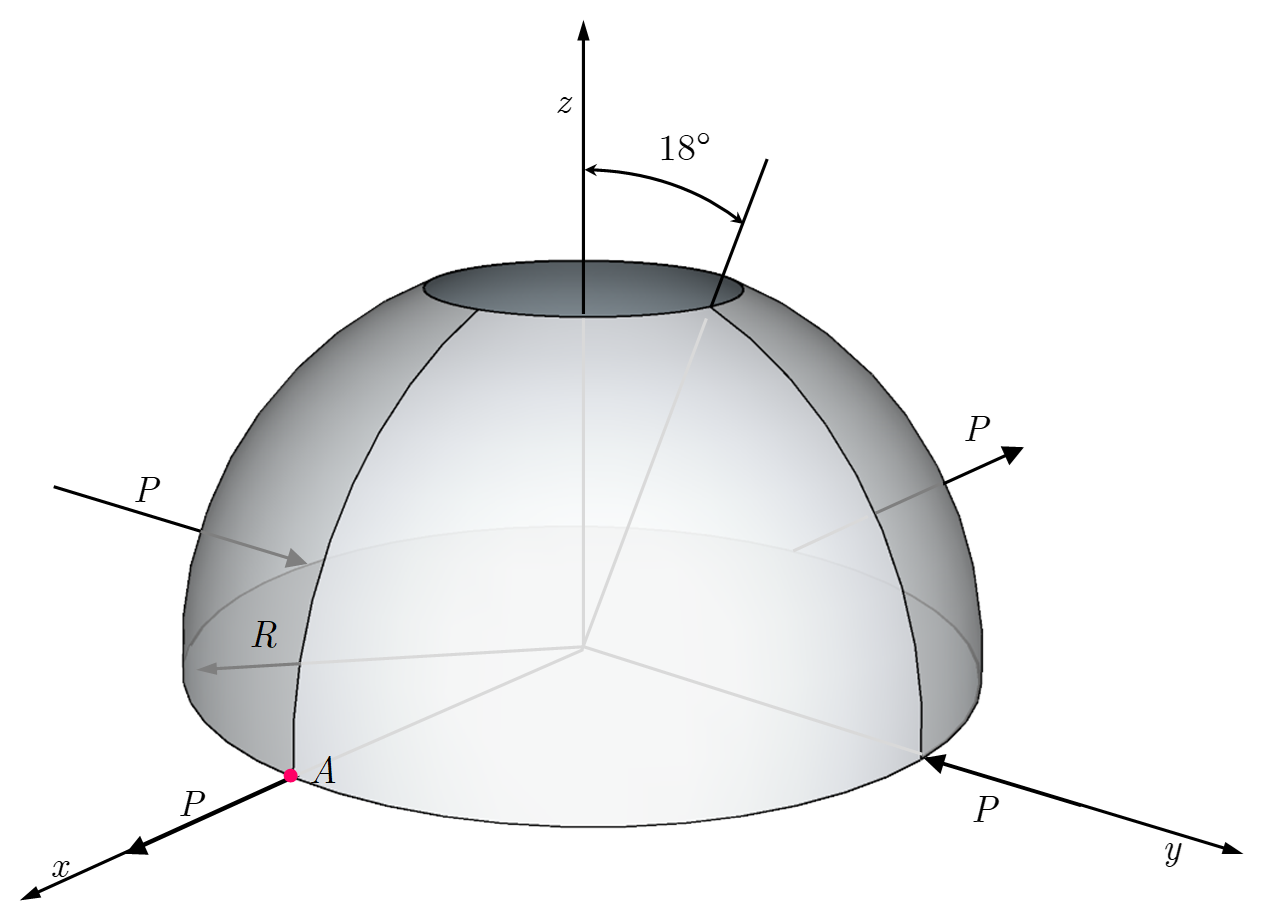
\includegraphics[width=0.8\textwidth]{figures/pfm}
\caption{Description of pinched hemispherical shell problem.}\label{phf1}
\end{figure}
\begin{figure}[!ht]
\centering
\DIFdelbeginFL %DIFDELCMD < 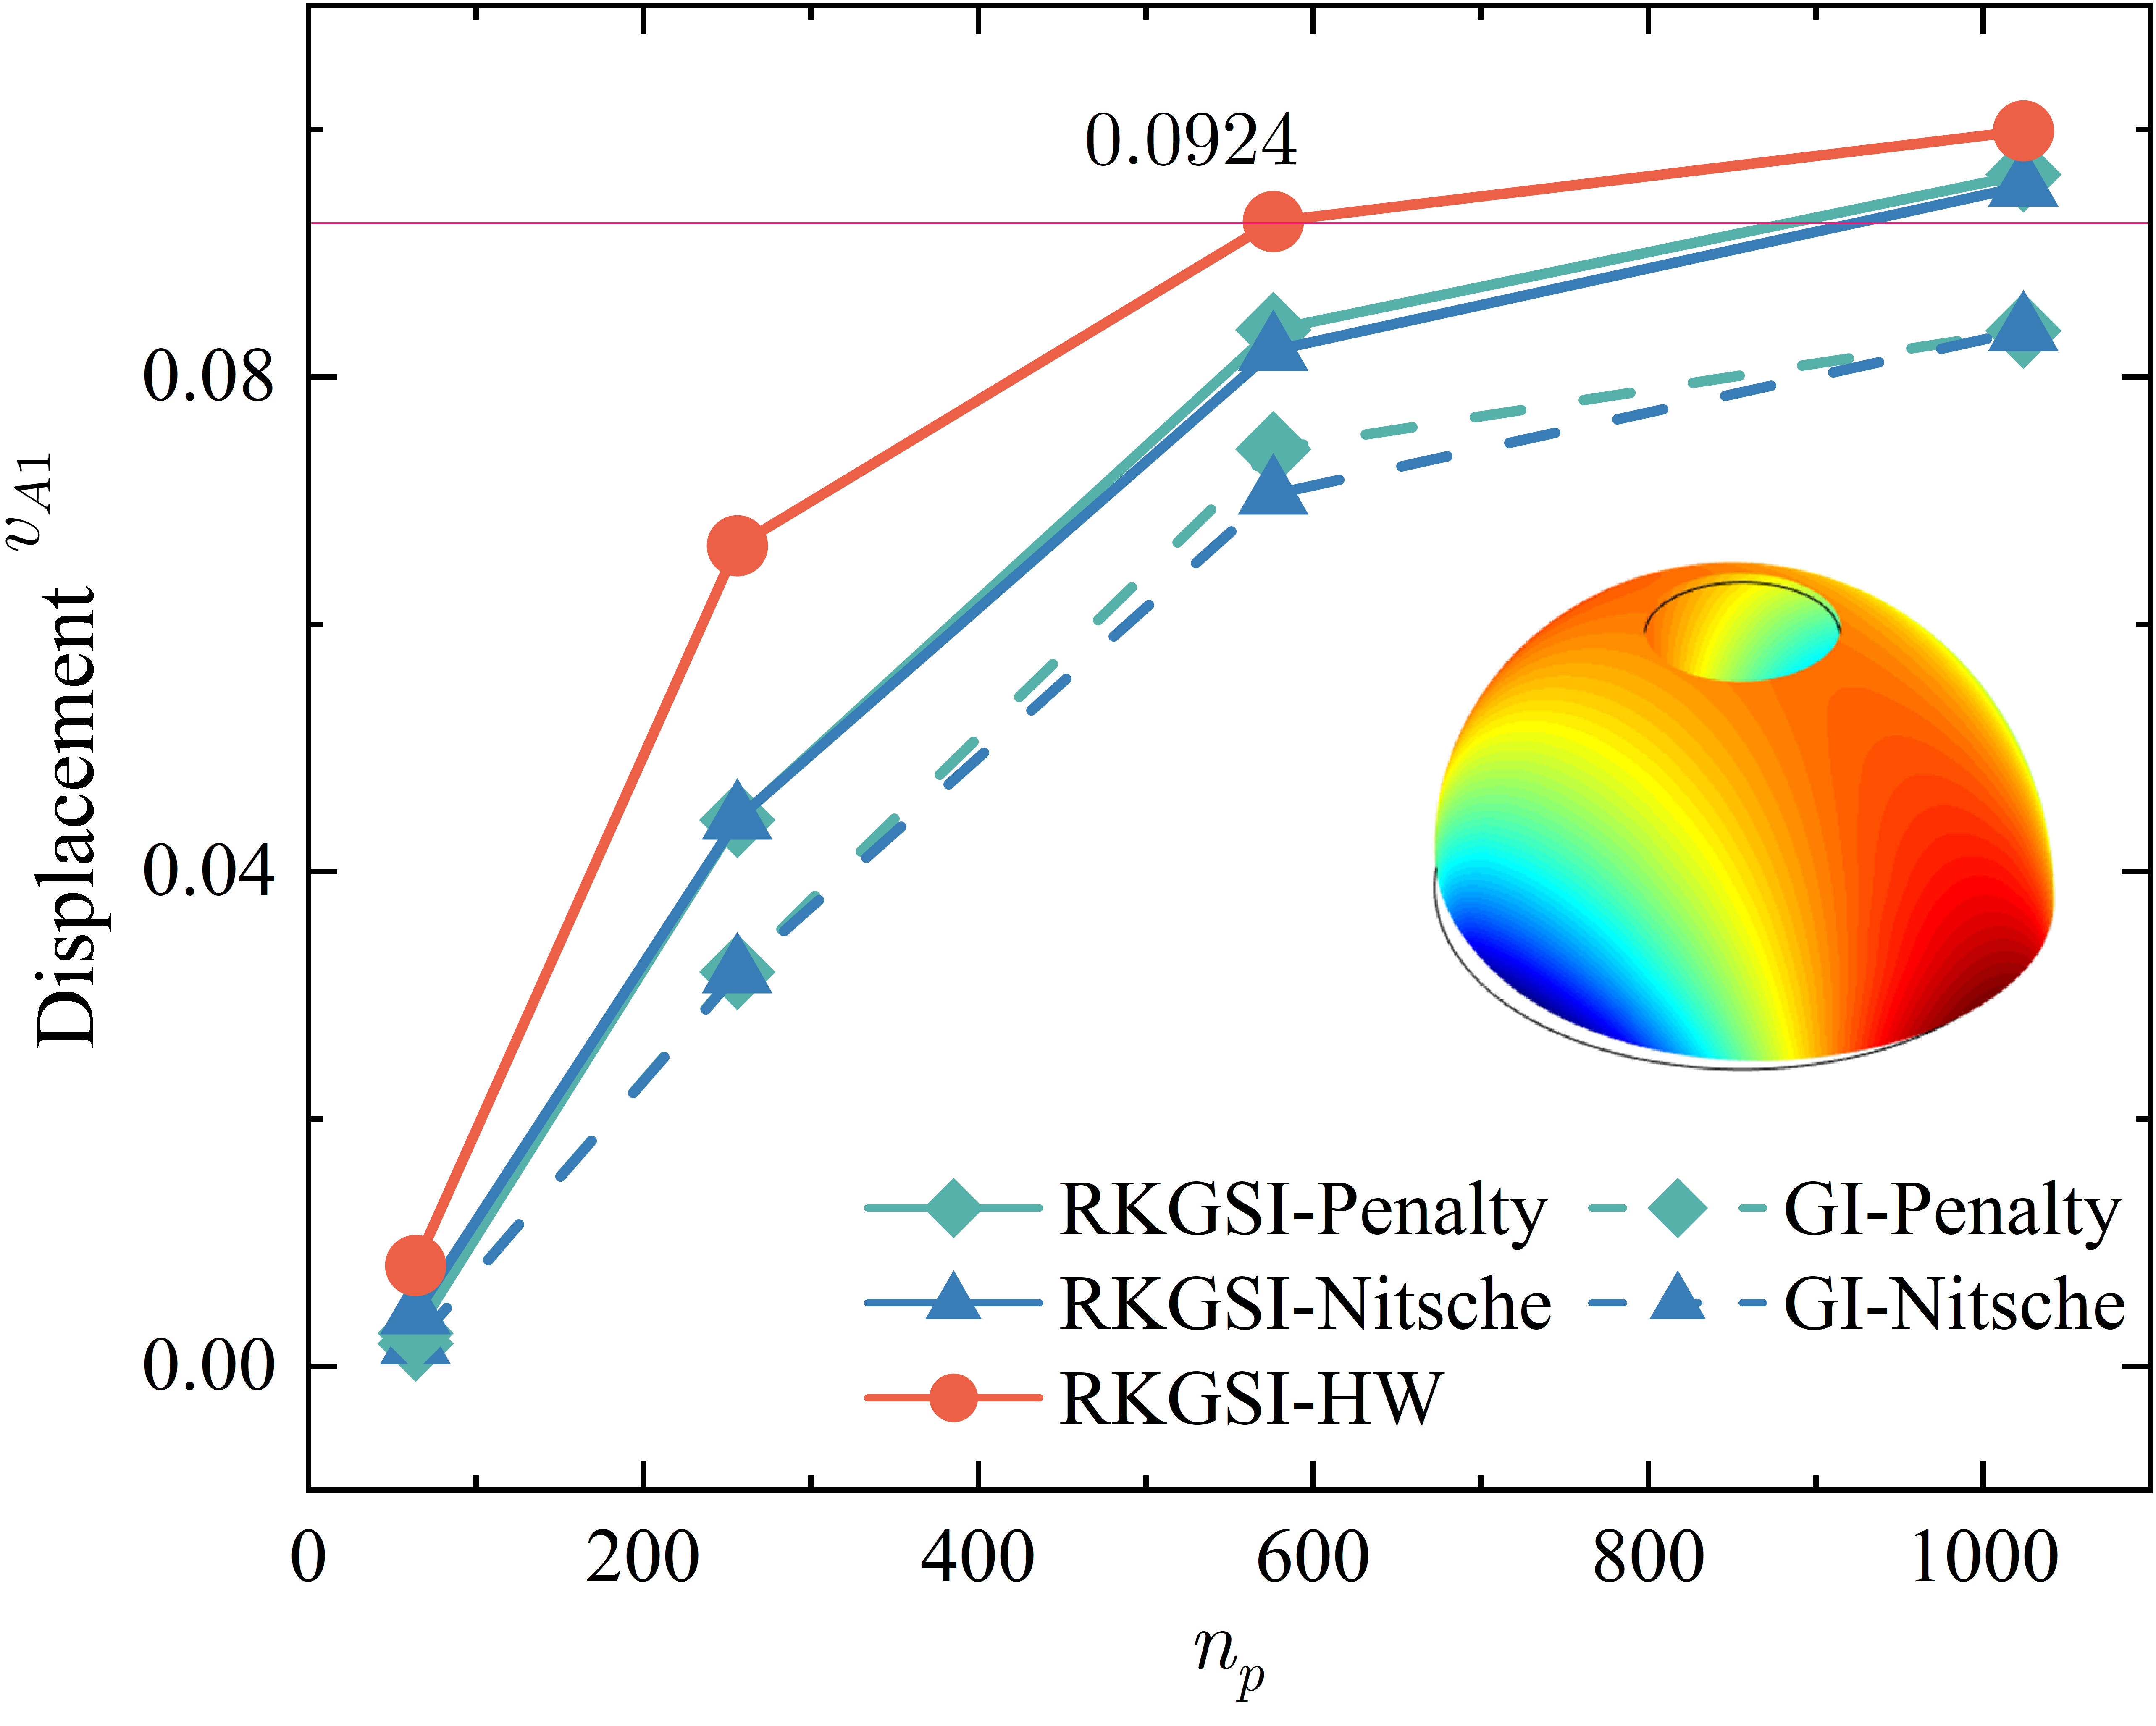
\includegraphics[width=\textwidth]{figures/pfd}
%DIFDELCMD < %%%
\DIFdelendFL \DIFaddbeginFL 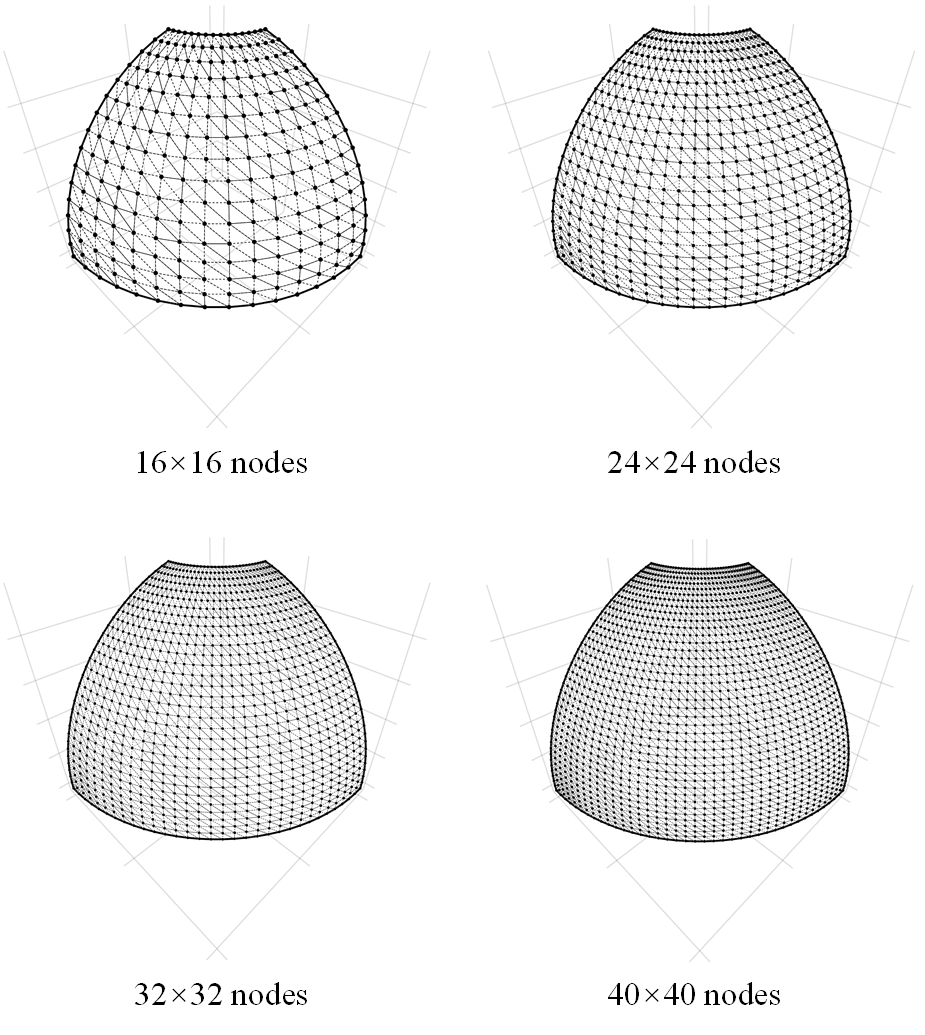
\includegraphics[width=\textwidth]{figures/pfmsh_r1}
\caption{\DIFaddFL{Meshfree discretizations for pinched hemispherical shell problem.}}\label{phfm}
\end{figure}
\begin{figure}[!ht]
\centering
\DIFdelbeginFL %DIFDELCMD < 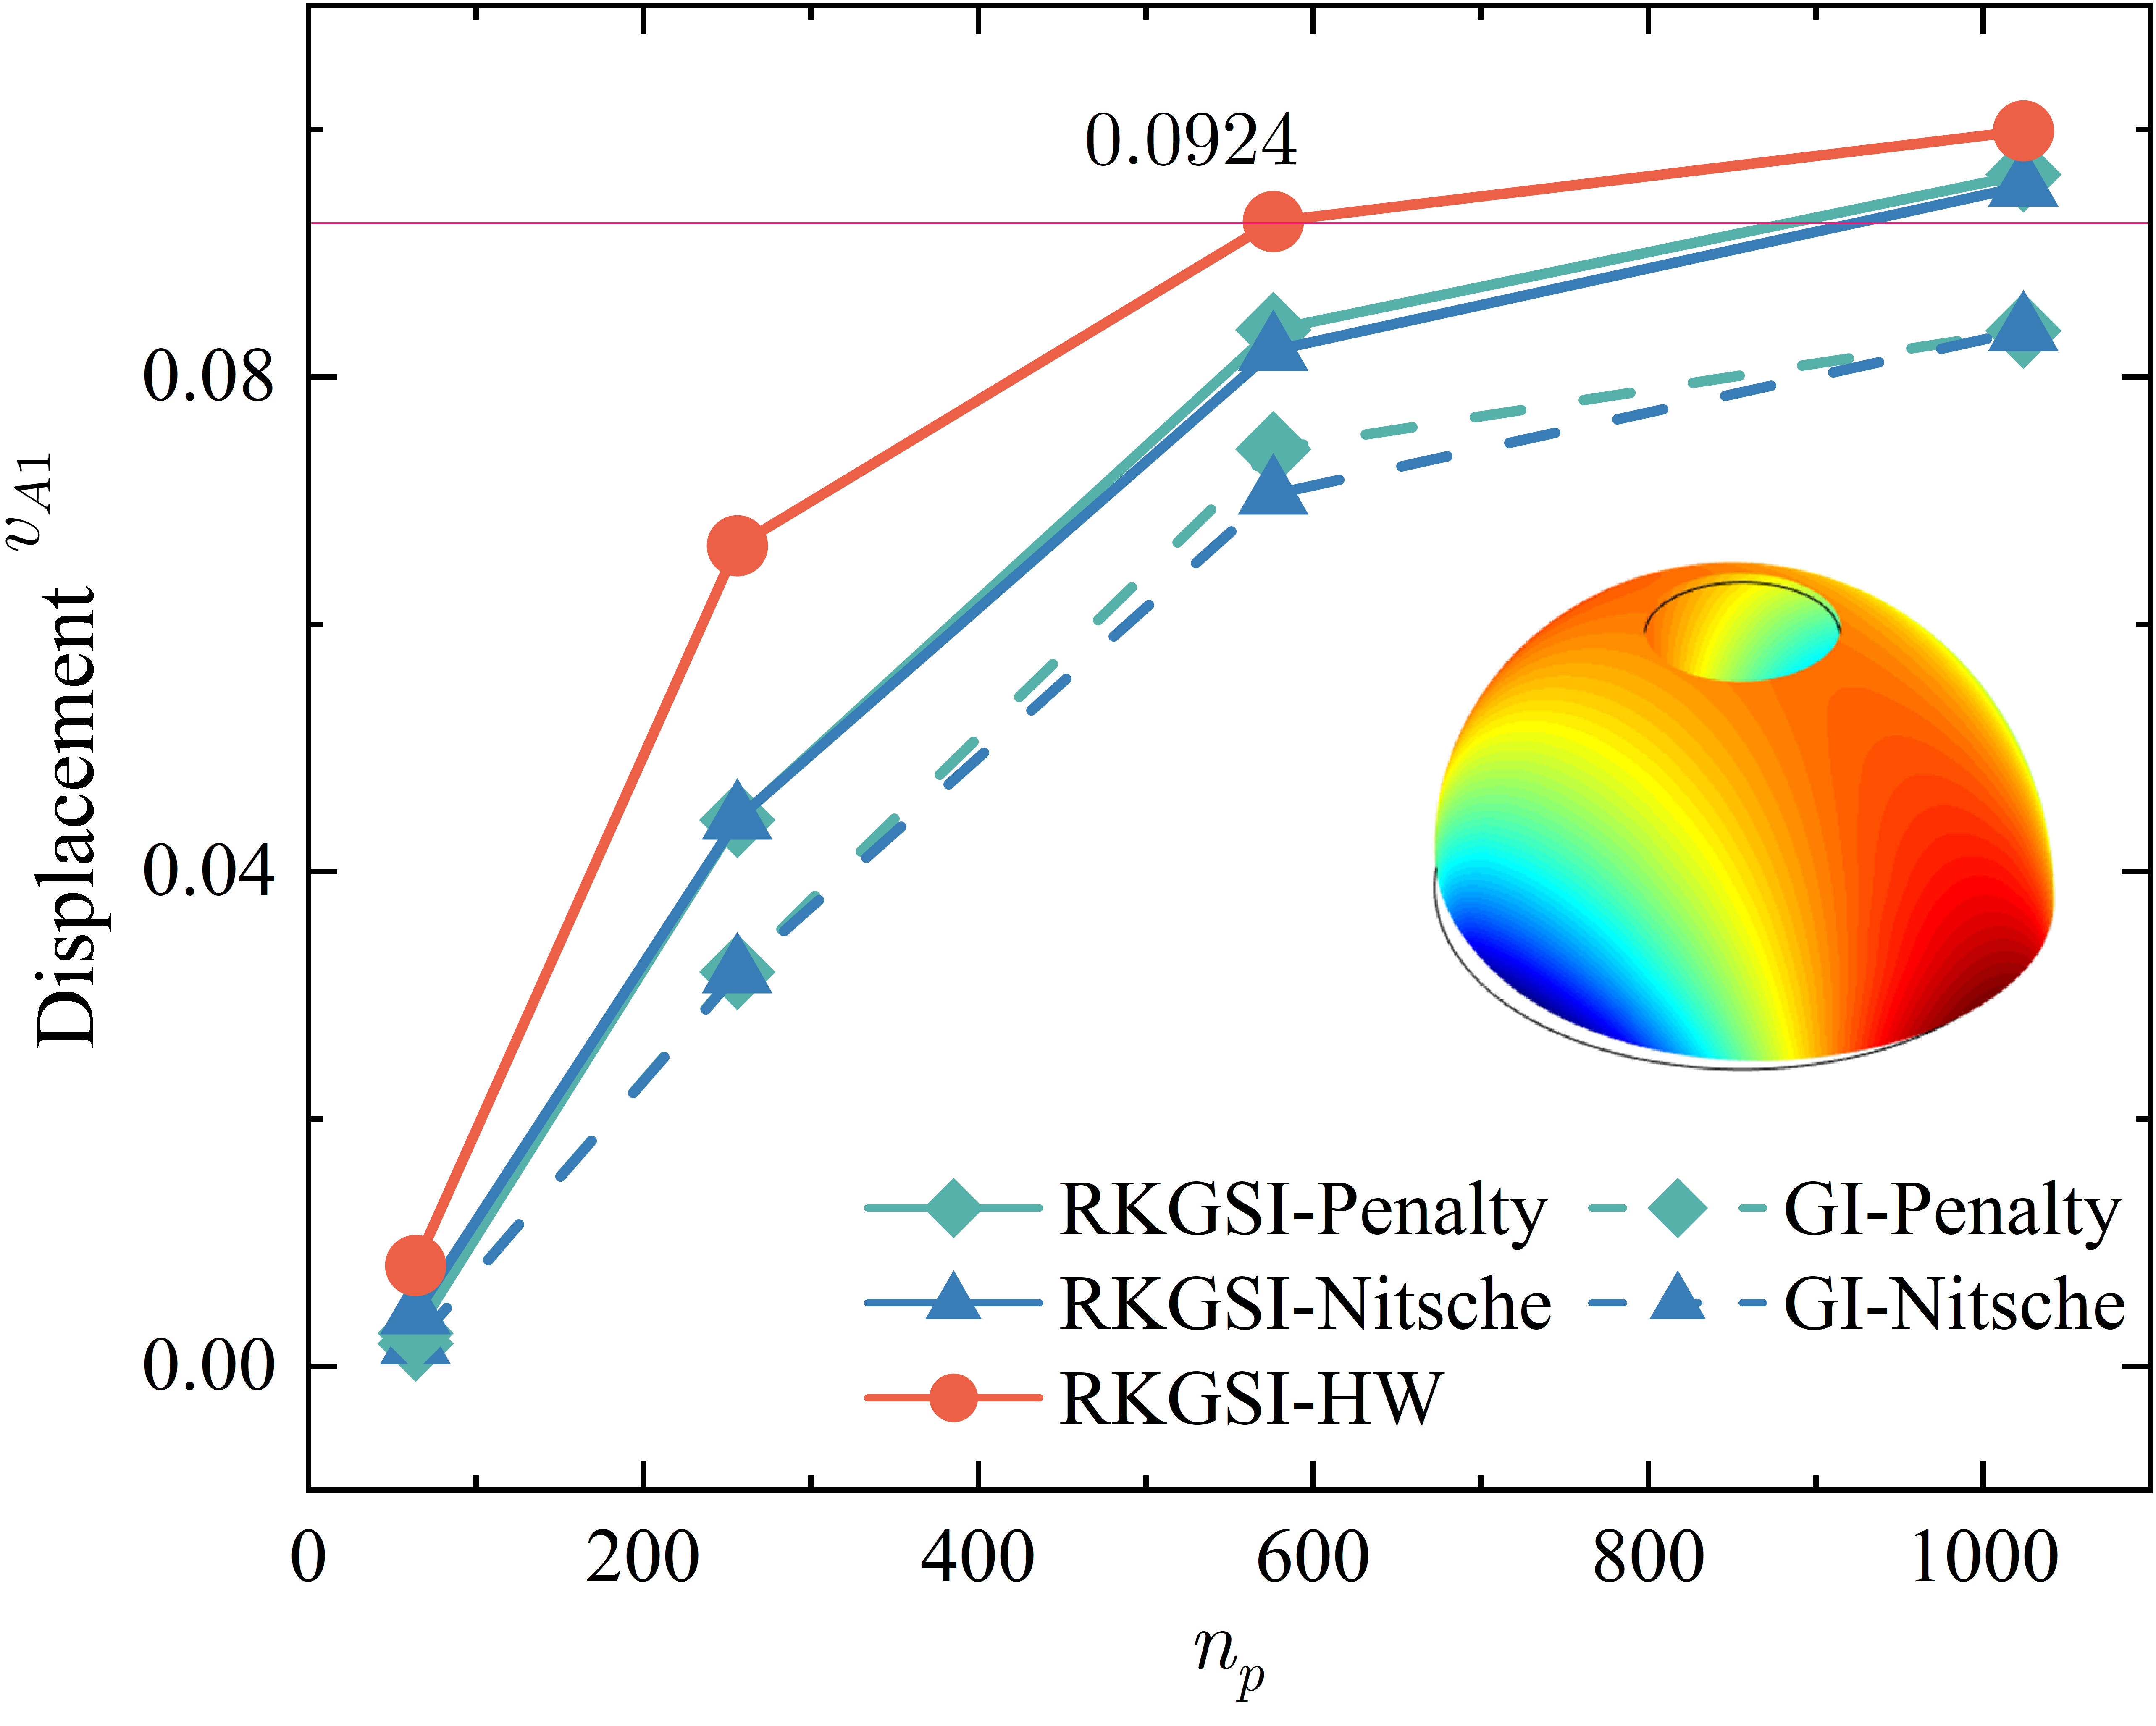
\includegraphics[width=\textwidth]{figures/pfd}
%DIFDELCMD < %%%
\DIFdelendFL \DIFaddbeginFL 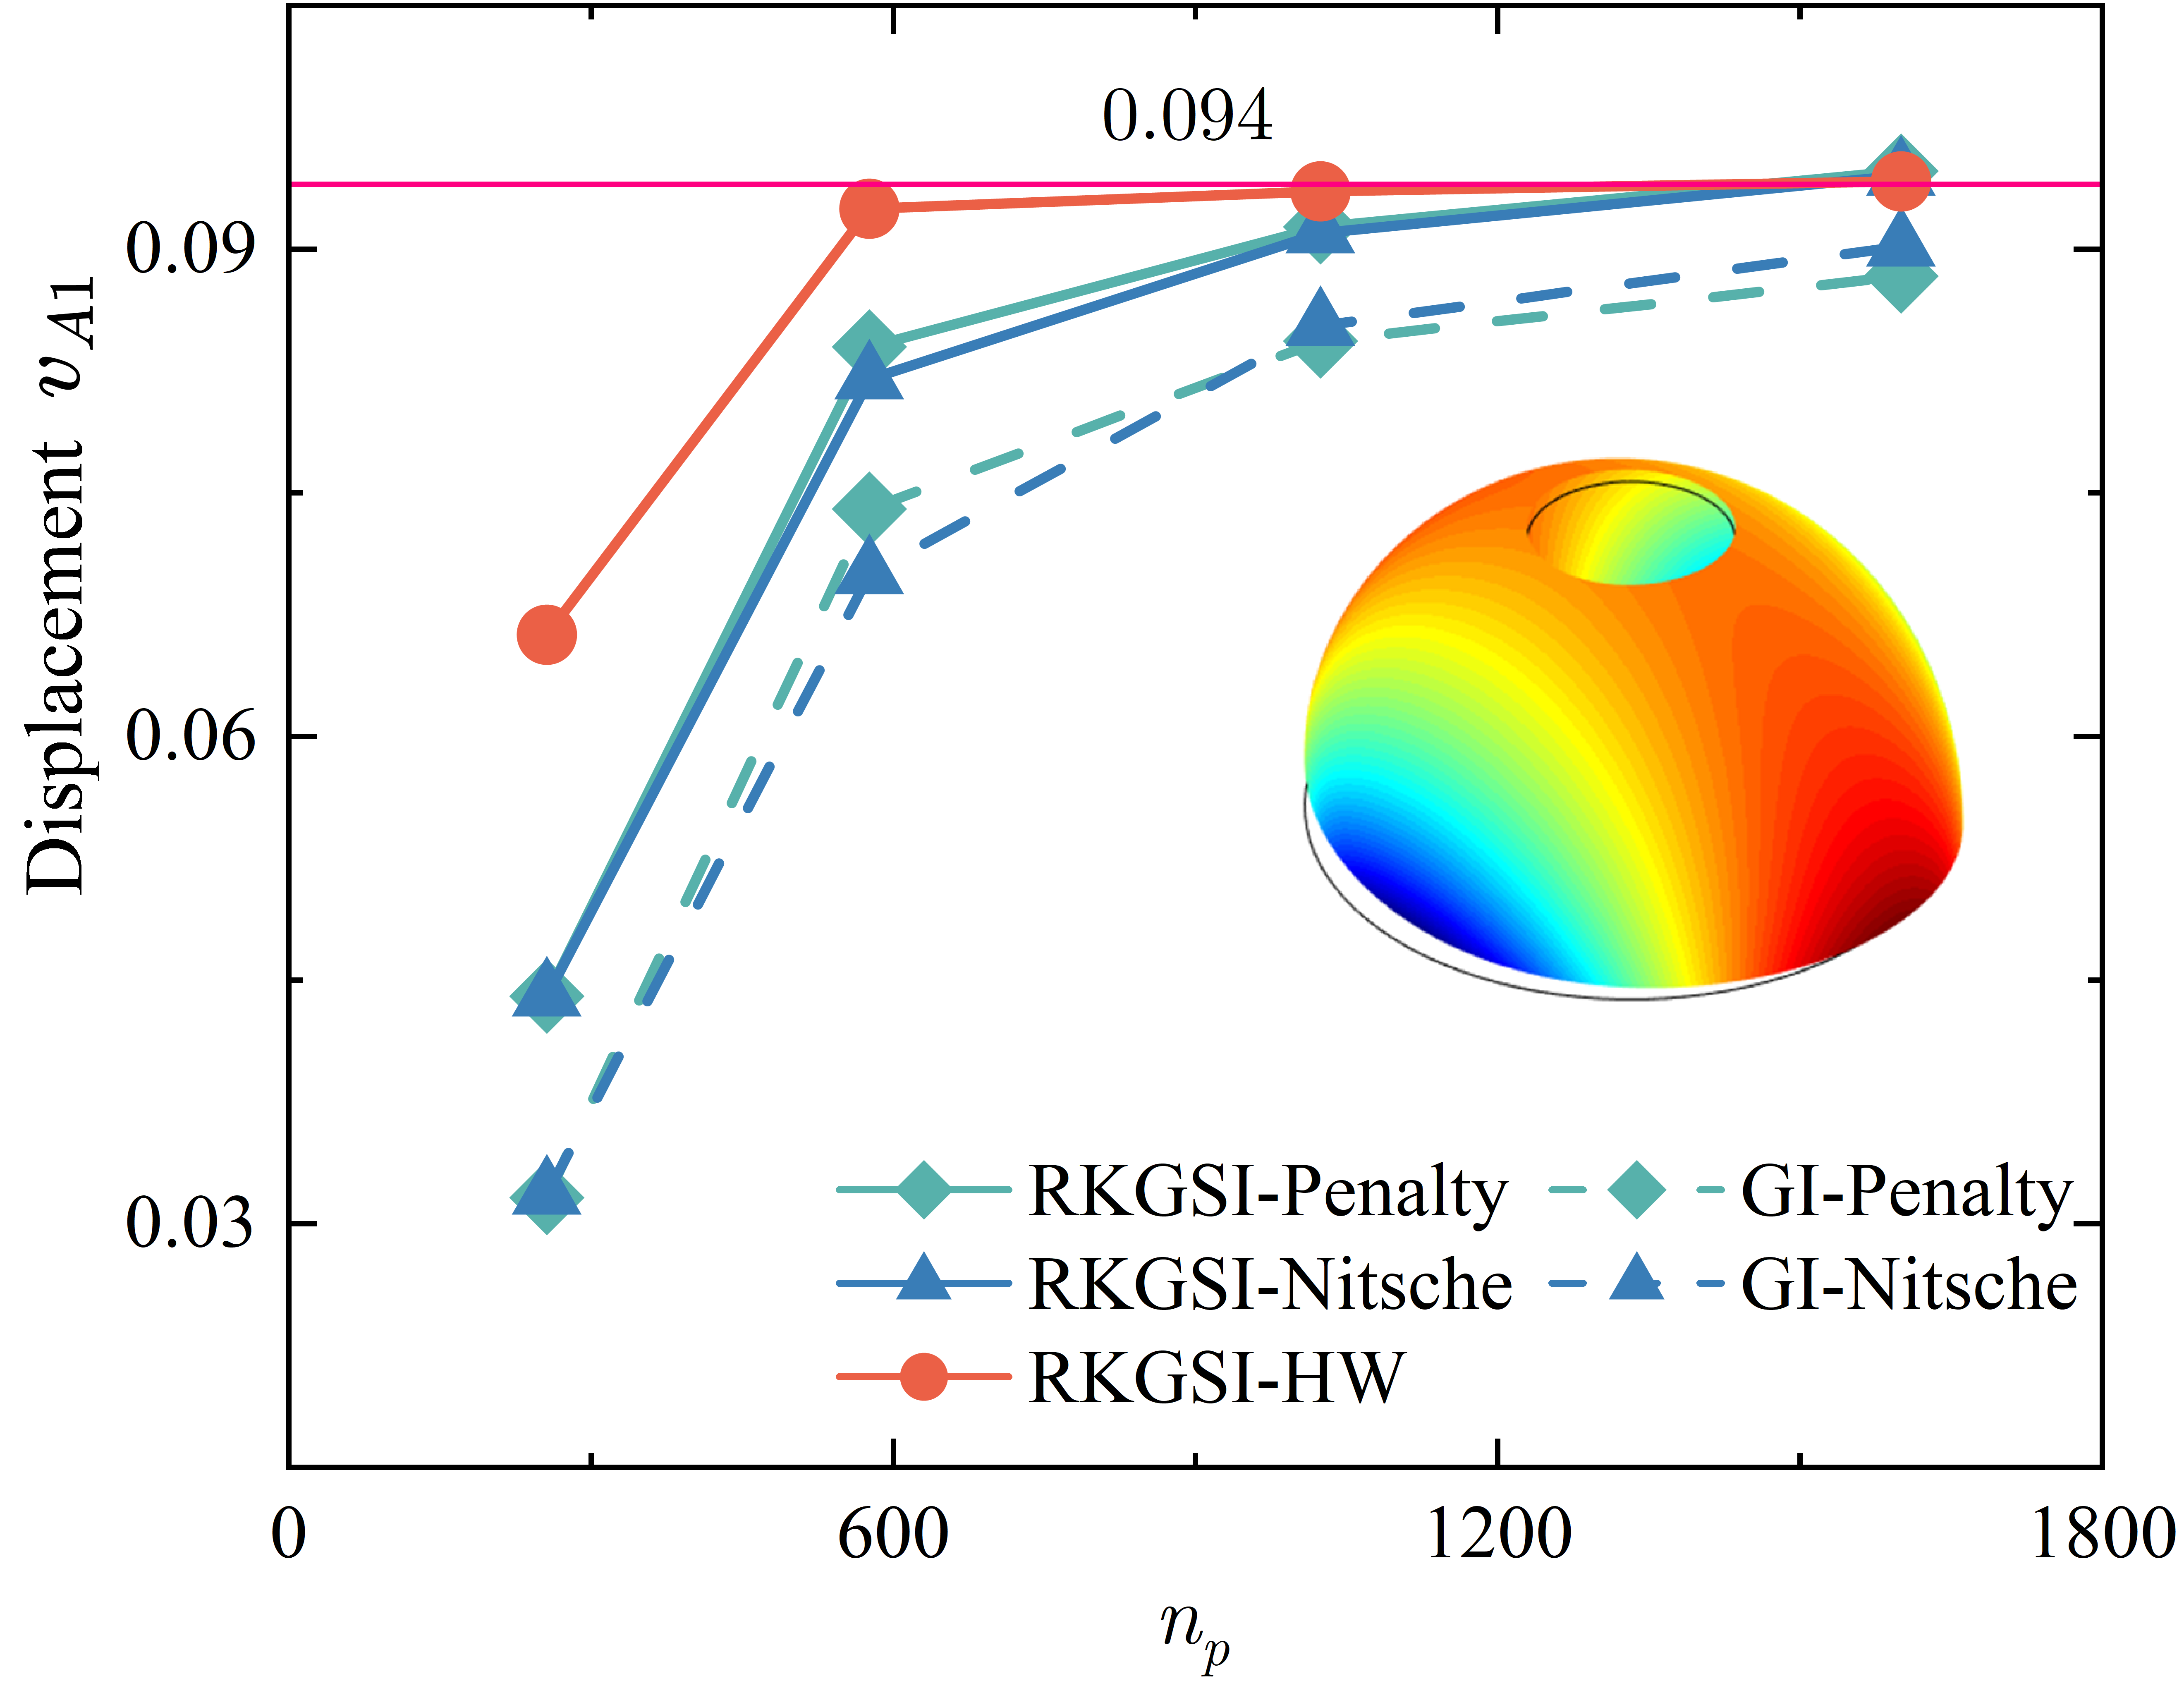
\includegraphics[width=\textwidth]{figures/pfd_r1}
\DIFaddendFL \caption{Displacement convergence for pinched hemispherical shell problem.}\label{phf2}
\end{figure}
\begin{figure}[!ht]
\centering
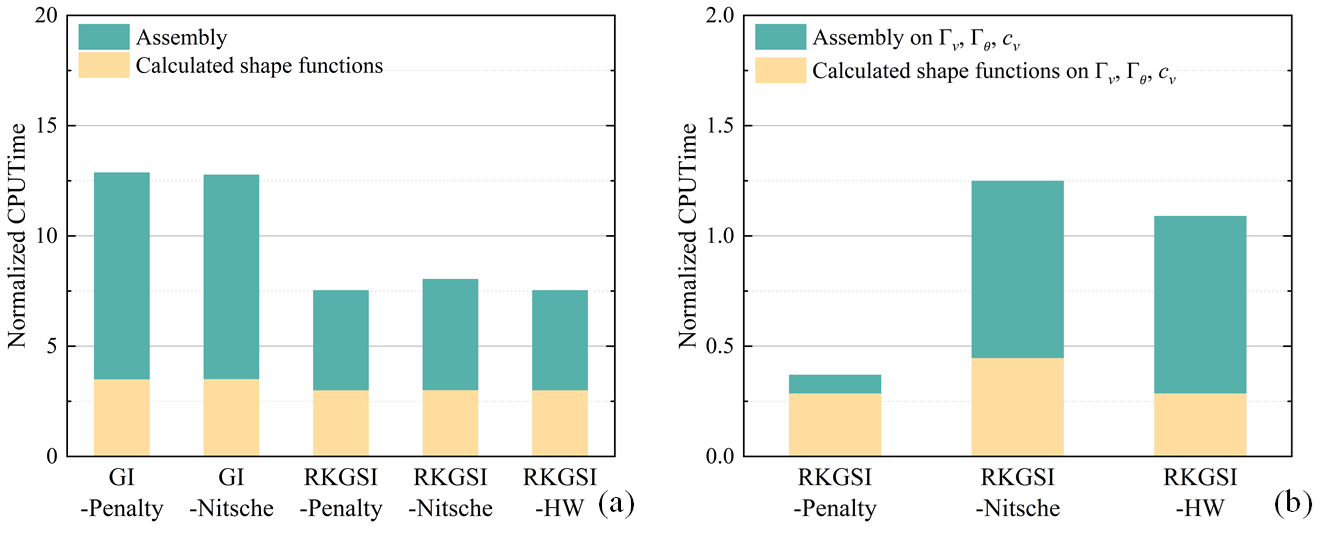
\includegraphics[width=\textwidth]{figures/efficient}
\caption{\DIFdelbeginFL \DIFdelFL{efficiency }\DIFdelendFL \DIFaddbeginFL \DIFaddFL{Efficiency }\DIFaddendFL comparison for pinched hemispherical shell problem: (a) Whole domain; (b) Essential boundaries}\label{phf3}
\end{figure}


